\chapter{Úvod do problematiky}

\section{Řídké matice}

% see: https://www.youtube.com/watch?v=jECBfI52hk8

Pro výstavu v roce 2011 s názvem Art in Enginnering v Harnově Muzeu představila floridská univerzita kolekci ilustrací řídkých matic s názvem The Beauty of Mathematics: As Illustrated by the University of Florida Sparse Matrix Collection \cite{Davis:2011:UFS:2049662.2049663}. Pro estetické zobrazení řídkých matic byla provedena simulace \cite{simul}. Každému uzlu byl přiřazen elektrický náboj a každá hrana představovala pružinu. V simulaci byla celá tato konstrukce položena na tvrdou podložku. Simulace byla zastavena v okamžiku, kdy se konstrukce přestala hýbat. Pro ilustraci přikládáme výsledek simulace \ref{fig:commanche} na modelu helikoptéry, tedy neorientovaném 3D grafu uloženém v řídké matici.

\begin{figure}
	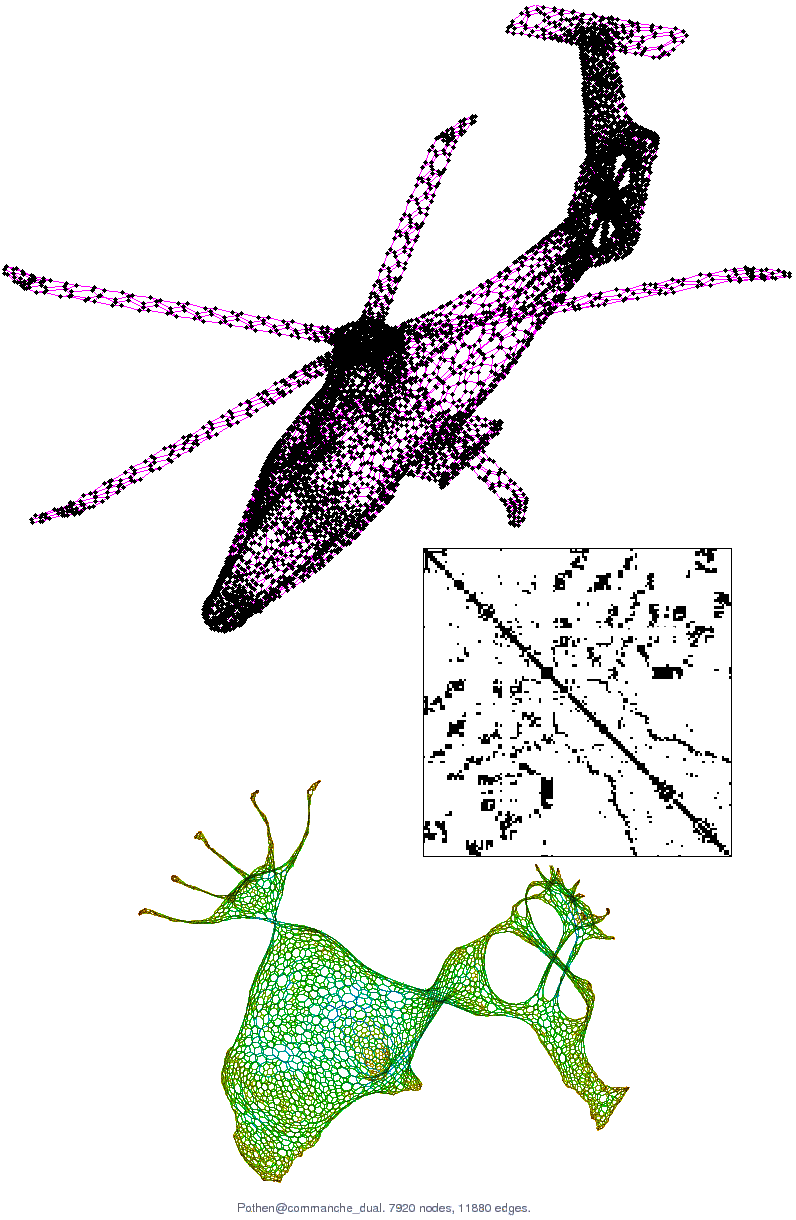
\includegraphics[width=1.0\textwidth]{./images/commanche/commanche}
	\caption{3D neorientovaný graf ve tvaru helikoptéry, jeho reprezentace v řídké matici a výsledek simulace}
	\label{fig:commanche}
\end{figure}

Řídké matice jsou používané ve velké škále oblastí \cite{sparsesw}, například výpočty diferenciálních rovnic, Google page rank, 3D grafika, statistika, těžení z dat, kryptografie a další.

% Použití řídkých matic najdeme 2D/3D grafice, simulaci fyzikálních jevů ať už řešení úloh proudění tekutin, elektrické či meteorologické, statistice, počítání pageranku % a další.
% TODO přeložit: computational fluid dynamics, finite-element methods, statistics, time/frequency 
% domain circuit simulation, dynamic and static modeling of chemical processes, 
% cryptography, magneto-hydrodynamics, electrical power systems, differential
% equations, quantum mechanics, structural mechanics (buildings, ships, aircraft,
% human body parts...), heat transfer, MRI reconstructions, vibroacoustics, linear 
% and non-linear optimization, financial portfolio optimization, semiconductor 
% process simulation, economic modeling, oil reservoir modeling, astrophysics, 
% crack propagation,  Google page rank, 3D computer vision, cell phone tower 
% placement, tomography, multibody simulation, model reduction, nano-technology, 
% acoustic radiation, density functional theory, quadratic assignment, elastic 
% properties of crystals, natural language processing, DNA electrophoresis, ... 

\section{Použití násobení matic}

Násobení maticí může znázorňovat nějakou transformaci jednoho stavu do druhého. Největší uplatnění řídkých matic je tedy v simulaci jevů, například fyzikálních, biologických, chemických, ekonomických a dalších. 

Jako příklad simulace můžeme uvést metodu konečných prvků \cite{4020926}\cite{0967-3334-30-6-S01}.

% http://ocw.mit.edu/courses/materials-science-and-engineering/3-11-mechanics-of-materials-fall-1999/modules/fea.pdf
% http://engineering.dartmouth.edu/~d22888z/documents/EIT_Bath_2011_v2.pdf

Pokud potřebujeme vynásobit jednu matici s více vektory, můžeme vektory složit do matice a provést násobení matice s maticí. To se hodí například v real-time aplikacích.

%psal to tady: http://www.researchgate.net/post/Could_anybody_tell_me_some_models_or_applications_in_which_Sparse_Matrix_Matrix_Products_are_required3
%ale dava to smysl

% \url{http://math.stackexchange.com/questions/116717/can-a-basis-for-a-vector-space-be-made-up-of-matrices-instead-of-vectors}

%\url{http://www.cise.ufl.edu/research/sparse/}

% inverze matic: Matrix multiplication and matrix inversion ItA


\section{Matice}

Matice \textbf{A} typu ($m$, $n$) je $m n$ uspořádaných prvků z množiny $\mathbf{R}$. O prvku $a_{r,s} \in \mathbf{R}, r \in \{1,2,\hdots,m\},s \in \{1,2,\hdots,n\}$ říkáme, že je na r-tém řádku a~s-tém sloupci matice \textbf{A}. Matici \textbf{A} zapisujeme do řádků a~sloupců takto:
\begin{align}
\mathbf{A}=\begin{pmatrix}
a_{1,1} & a_{1,2} & \cdots & a_{1,n} \\
a_{2,1} & a_{2,2} & \cdots & a_{2,n} \\
\vdots  & \vdots  & \ddots & \vdots  \\
a_{m,1} & a_{m,2} & \cdots & a_{m,n}
\end{pmatrix}
\end{align}

Matici \textbf{M} typu ($m$, $n$), kde všechny její prvky jsou rovny nule, nazýváme \textit{nulovou maticí.}

O~matici typu ($m$, $n$) budeme říkat, že je $m$~široká a~$n$~vysoká. Pokud o~matici řekneme, že má velikost $n$, myslíme tím, že je typu ($n$, $n$).

\section{Vektor}

Matici \textbf{V} typu (1, n) nazveme vektorem.

\section{Definice násobení matice maticí}
\label{defmmm}

Buď \textbf{A} matice typu ($m$,$n$) s prvky $a_{i,j}$ a \textbf{B} matice typu ($n$,$p$) s prvky $b_{j,k}$. Definujeme součin matic $\mathbf{A} \cdot \mathbf{B}$ jako matici \textbf{C} typu ($m$,$p$) s prvky $c_{i,k}$, které vypočteme jako:

\begin{align}
c_{row,col}=\sum_{k=1}^{N} a_{row,k} \cdot b_{k,col}
\end{align}

Výsledek součinu matic se nezmění, pokud matice doplníme o~libovolný počet nulových řádků a~nebo sloupců. Této vlastnosti můžeme využít pro získání potřebných rozměrů:

\begin{enumerate}
  \item Při násobení matice A typu ($m$,$n$) s maticí B typu ($o$,$p$), kde $ n \neq o $.
  \item Pokud potřebujeme matice stejné velikosti.
  \item Pokud potřebujeme matice určité velikosti, například $ 2^{ \mathbf{N}} $.
\end{enumerate}

Násobení matice vektorem je pouze případem násobení matice typu ($m$,$n$) s maticí typu ($1$,$n$).

\section{Složitosti}

K označení složitostí, ať již časových nebo prostorových (paměťových), používáme \bigO-notaci, která označuje množinu funkcí, asymptoticky rostoucí řádově stejně rychle nebo rychleji.
\begin{align}
\bigO(g(n)) = \left\{ f(n) : \exists c \in R^+ \exists n_0 \in N \forall n \geq n_0 : 0 \leq f(n) \leq cg(n) \right\}
\end{align}
\bigO\texttt{ }notací budeme popisovat nejhorší možný případ. Obdobně $\Theta$ značí funkce rostoucí stejně rychle a $\Omega$ stejně rychle nebo pomaleji.

% IntroductionToAlgoritms 3.1 asymptotic notations 43-97 (1217, 1222).

Pro výpočet složitostí rekurzivních algoritmů používáme mistrovskou metodu \cite{Cormen:2001:IA:580470}. Pokud $a \geq 1, b > 0$ jsou konstanty a $f(n)$ je funkce o jedné proměnné, tak rekurence

\begin{align}
t(n) = at(n/b)+f(n)
\end{align}

má asymptotickou složitost:

\begin{enumerate}
  \item Pro $f(n) = \bigO(n^{log_b{a - \epsilon}})$, kde $\epsilon > 0$ je konstanta platí, že $t(n)=\Theta(n^{log_b{a}})$.
  \item Pro $f(n) = \Theta(n^{log_b{a}})$ platí, že $t(n)=\Theta(n^{log_b{a}}log{n})$.
  \item Pro $f(n) = \Omega(n^{log_b{a + \epsilon}})$, kde $\epsilon > 0$ je konstanta a $af(n/b) \leq cf(n)$ pro konstantu $c < 1$ a $\forall n\geq n_0$, tak platí, že $t(n)=\Theta(f(n))$.
\end{enumerate}

\section{Řídké matice}

Matice, které obsahují velké množství nulových prvků, nazýváme řídké. Nebudeme přesně uvádět, kolik procent z celkového počtu prvků musí být nulových, abychom matici nazývali řídkou. Stejně jako řídkou matici můžeme uložit do formátu pro husté matice, můžeme hustou matici uložit do formátu pro řídké matice.

Řídkost matice budeme vyjadřovat pomocí $nnz$ (Number of NonZero elements), tedy počtem nenulových prvků z celkových $mn$, pro matici A typu ($m$, $n$).

%\section{Typy řídkých matic}
%TODO: typy ridkych matic (pasova, atd, pattern, real)

% \section{Numerická stabilita}

% TODO: numerická stabilita obecne (viz strassen)

% \section{Optimalizace kódu}

% Dnešní překladače umí velice dobře optimalizovat vygenerovaný kód. Pokusy o nějaké mikrooptimalizace program spíše zpomalí.

% Je vhodné používat funkce standartních knihoven, protože bývají optimalizované přímo v assembleru.

% TODO: priklady, zdroje

% \subsection{Rozděl a panuj}
% divide, conquer, combine

% \subsection{Rozbalování cyklů}

% \subsection{AoS -> SoA}

% \subsection{Loop tiling}

% TODO: \url{https://edux.fit.cvut.cz/courses/BI-EIA/_media/lectures/kompilator.pdf}

%-----------------------------------------------------------------------------
%-----------------------------------------------------------------------------
%-----------------------------------------------------------------------------